\documentclass[11pt]{article}

%	packages
\usepackage{tikz}
\usepackage{authblk}
\usepackage{amsmath}
\usepackage{amssymb} 
\usepackage{caption}
\usepackage{graphicx}
\usepackage[hypertexnames=false,colorlinks=true,linkcolor=blue,citecolor=blue]{hyperref}
\usepackage[numbers,comma,square,sort&compress]{natbib}
\usepackage[a4paper,text={6.5in,10in},centering]{geometry}
\usepackage{subcaption}
%	code syntax higlighting
\usepackage{listings}
\usepackage{color}
\usepackage{textcomp}
\definecolor{listinggray}{gray}{0.9}
\definecolor{lbcolor}{rgb}{0.9,0.9,0.9}
% C++ = [Visual]C++ ; matlab = matlab
\lstset{
	backgroundcolor=\color{lbcolor},
	tabsize=4,
	rulecolor=,
	language=java,
	keywordstyle=\bfseries\ttfamily\color[rgb]{0,0,1},
	identifierstyle=\ttfamily,
	commentstyle=\color[rgb]{0.133,0.545,0.133},
	stringstyle=\ttfamily\color[rgb]{0.627,0.126,0.941},
	showstringspaces=false,
	basicstyle=\small,
	%numberstyle=\footnotesize,
	%numbers=left,
	stepnumber=1,
	numbersep=10pt,
	tabsize=2,
	breaklines=true,
	prebreak = \raisebox{0ex}[0ex][0ex]{\ensuremath{\hookleftarrow}},
	breakatwhitespace=false,
	aboveskip={1.5\baselineskip},
  columns=fixed,
  upquote=true,
  extendedchars=true,
 frame=single,
% backgroundcolor=\color{lbcolor},
}


%	figures
\graphicspath{{eps/}{pdf/}{../figs//}}
%\setcaptionmargin{0.25in}
\def\captionfont{\itshape\small}
\def\captionlabelfont{\upshape\small}

%	counters
\makeatletter\@addtoreset{equation}{section}\makeatother
\renewcommand{\theequation}{\arabic{section}.\arabic{equation}}


%%%%%%%%%%%%%%%%%%%%%%%%%%%%%%%%%%%%%%%%%%%%%%%%%%%%%%%%%%%%%%%%%%%%%%%%%%%%

\begin{document}

\title{Equation-free analysis of agent-based models:\\Altruism Model}

%\author[1]{Spencer A. Thomas}
\author{Spencer A. Thomas}
\author{David J.B. Lloyd}
\author{Anne C. Skeldon}
%\affil[1]{\small Department of Mathematics, Evolution and Resilience of Industrial Ecosystems (ERIE), University of Surrey, Guildford, GU2 7XH, UK}
\affil{\small Department of Mathematics, Evolution and Resilience of Industrial Ecosystems (ERIE), University of Surrey, Guildford, GU2 7XH, UK}
\date{\today}
\maketitle


%%%%%%%%%%%%%%%%%%%%%%%%%%%%%%%%%%%%%%%%%%%%%
% stochastic double well
%%%%%%%%%%%%%%%%%%%%%%%%%%%%%%%%%%%%%%%%%%%%%

\section{The Model: An Overview}
The altruism model \cite{Altruism} simulates the competition between selfish and altruistic agents for survival in a 2D world. This model is available from the NetLogo model library \cite{Netlogo}. In general the outcome of this battle depends on the environmental conditions (parameters) though there is a stochastic element coming from the initial configuration of the system, i.e. the randomised positioning of the agents. The system is randomly initialised where each space element in the 2D lattice has a defined probability of being either selfish, altruistic or empty. Selfish and altruists compete for occupation of positions in the world based on simple rules but leading to some complex behaviour and non linear dynamics. 


\begin{figure}[h]
        \centering
        		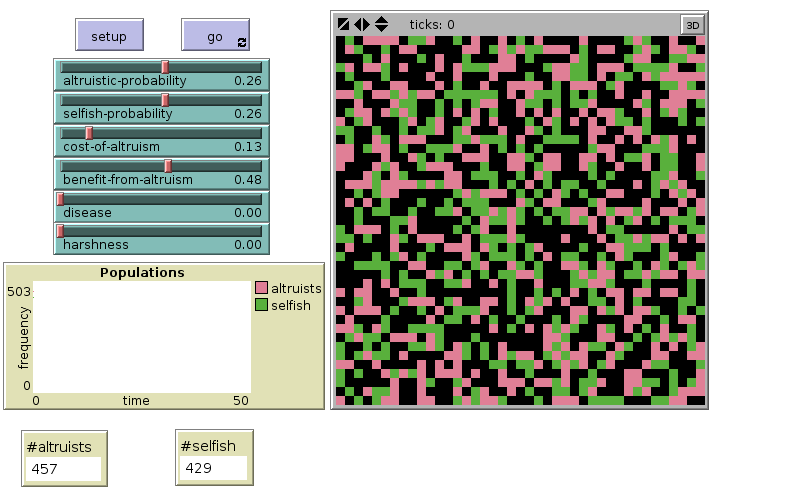
\includegraphics[width=\textwidth]{AltruismInterface.png}
        \caption{Altruism interface with several controllable parameter.\label{altruism}}
\end{figure}



\section{The Model: Details} 
\label{sec:details}
In this model agents are patches in the 2D lattice and compete for occupation of space in the world. In this  model groups of five agents, a central agent and its surrounding neighbours, compete for occupation of the central patch. The world wraps around such that an agent on the `edge' of the world have neighbours on the opposite edge, thus there is a continuous flow of agents and neighbours. The occupation of the central location is based on the agents fitness values.  All agents have a fitness value calculated as;
	\begin{equation}
		F_A = 1 - C_A + \frac{\sum\limits^{nbh} N_A}{5} B_A~,
	\end{equation}	
	\begin{equation}
		F_S = 1  + \frac{\sum\limits^{nbh} N_A}{5} B_A~,
	\end{equation}
	\begin{equation}
		F_E = H~,
	\end{equation}
	where $F_A$, $F_S$ and $F_E$ are the fitness values for altruistic, selfish and empty agents respectively. Empty agents correspond to locations where there is neither an altruist or selfish agent. System parameters $C_A$, $B_A$ and $H$ represent the cost and benefits of altruism, and the harshness of the environment respectively. The term $\sum\limits^{nbh} N_A / 5$ is the average number of altruists in the neighbourhood ($nbh$), that is the central location and its four neighbours. At each unit of time an agent and its four neighbours use their fitness values to compete for occupation of the central location by using weighted probability, $P$, calculated as:
	\begin{equation}
		P_A = \frac{\sum\limits^{N_A} F_A}{F_T}~,
	\end{equation}	
	\begin{equation}
		P_S = \frac{\sum\limits^{N_S} F_S}{F_T}~,
	\end{equation}		
	\begin{equation}
		P_E = \frac{\sum\limits^{N_E} F_E + D}{F_T}~,
	\end{equation}
	where 
	\begin{equation}
		F_T = \sum\limits^{N_A} F_A + \sum\limits^{N_S} F_S + \sum\limits^{N_E} F_E + D~.
	\end{equation}
	Here $N_i$ is the number of $i$-type agents and $D$ is the rate of disease in the environment. Agents enter a lottery for the central position based on these seeds. A random number, $r$, is generated between 0 and 1, and the central position becomes; an altruist if $r<P_A$, selfish if $r<P_A+P_S$, and empty if $r>P_A+P_S$. This process continues at each time iteration for all locations simultaneously, which with the random initial configuration of agent location, leads to stochastic behaviour. There is a conservation in the model with the total number of patches, where patches can be either either Altruists or Selfish agents, or Voids. The relative number of each patch type must sum to unity, $N_A+N_S+N_V=1$, therefore the number of agents under any settings is confined to a plane in $g(N_A,N_S,N_V)$ space. . 

\newpage
\section{Requirements of the User}
The user defined settings in the input file are given below. 
\begin{lstlisting}
String NetlogoFile = "netlogo/Altruism.nlogo"; 
String[] systemParameters = {"set disease ", "set cost-of-altruism ", "set benefit-from-altruism ", "set harshness "};	
double[] param = {0.4, 0.13, 0.48, 0.85};		
String[] Measure		 = {"count patches with [pcolor = pink] / count patches ", "count patches with [pcolor = green] / count patches "};	
String[] LiftOperator  = {"set altruistic-probability ", "set selfish-probability "}; 
double[]xInitial = {0.5,	0.5};
boolean isSystemInitialised = false;
\end{lstlisting}		
	Here the {\tt NetlogoFile} is a string of text with the location of the NetLogo file, here contained in the sub-folder {\it netlogo}. {\tt Lift} is the name of the parameters required to set up with system, which correspond to the values in {\tt param}. Note the parameter you wish to vary in order to analyse the system with this package goes first in this list. {\tt systemParameters} are the parameters are the parameters you wish to monitor during this analysis which take the initial value of {\tt Initial} as an estimate of the first fixed point of the system. Note there can be any number of {\tt systemParameters} in your system. {\tt Measure} is the output measure of the system, note this is not the same as {\tt systemParameters} in general.

\section{Outcome of Equation-free Analysis}


In this model we continue in the disease parameters $D$ for several system configuration; 1) $N_S=0$ (no selfish agents), 2) $N_A=0$ (no altruistic agents) and 3) $N_S=0$ and $N_A=0$ (no agents) given in Fig.~\ref{fig:altruistBifurcation}. This illustrates the different dependence on $D$ with Altruistic and Selfish agents varying nonlinearly and linearly respectively. Additionally we can see that the two agents differ in stability, altruistic branch beginning unstable and the selfish branch beginning stable. 

\begin{figure}[t]
	\centering
	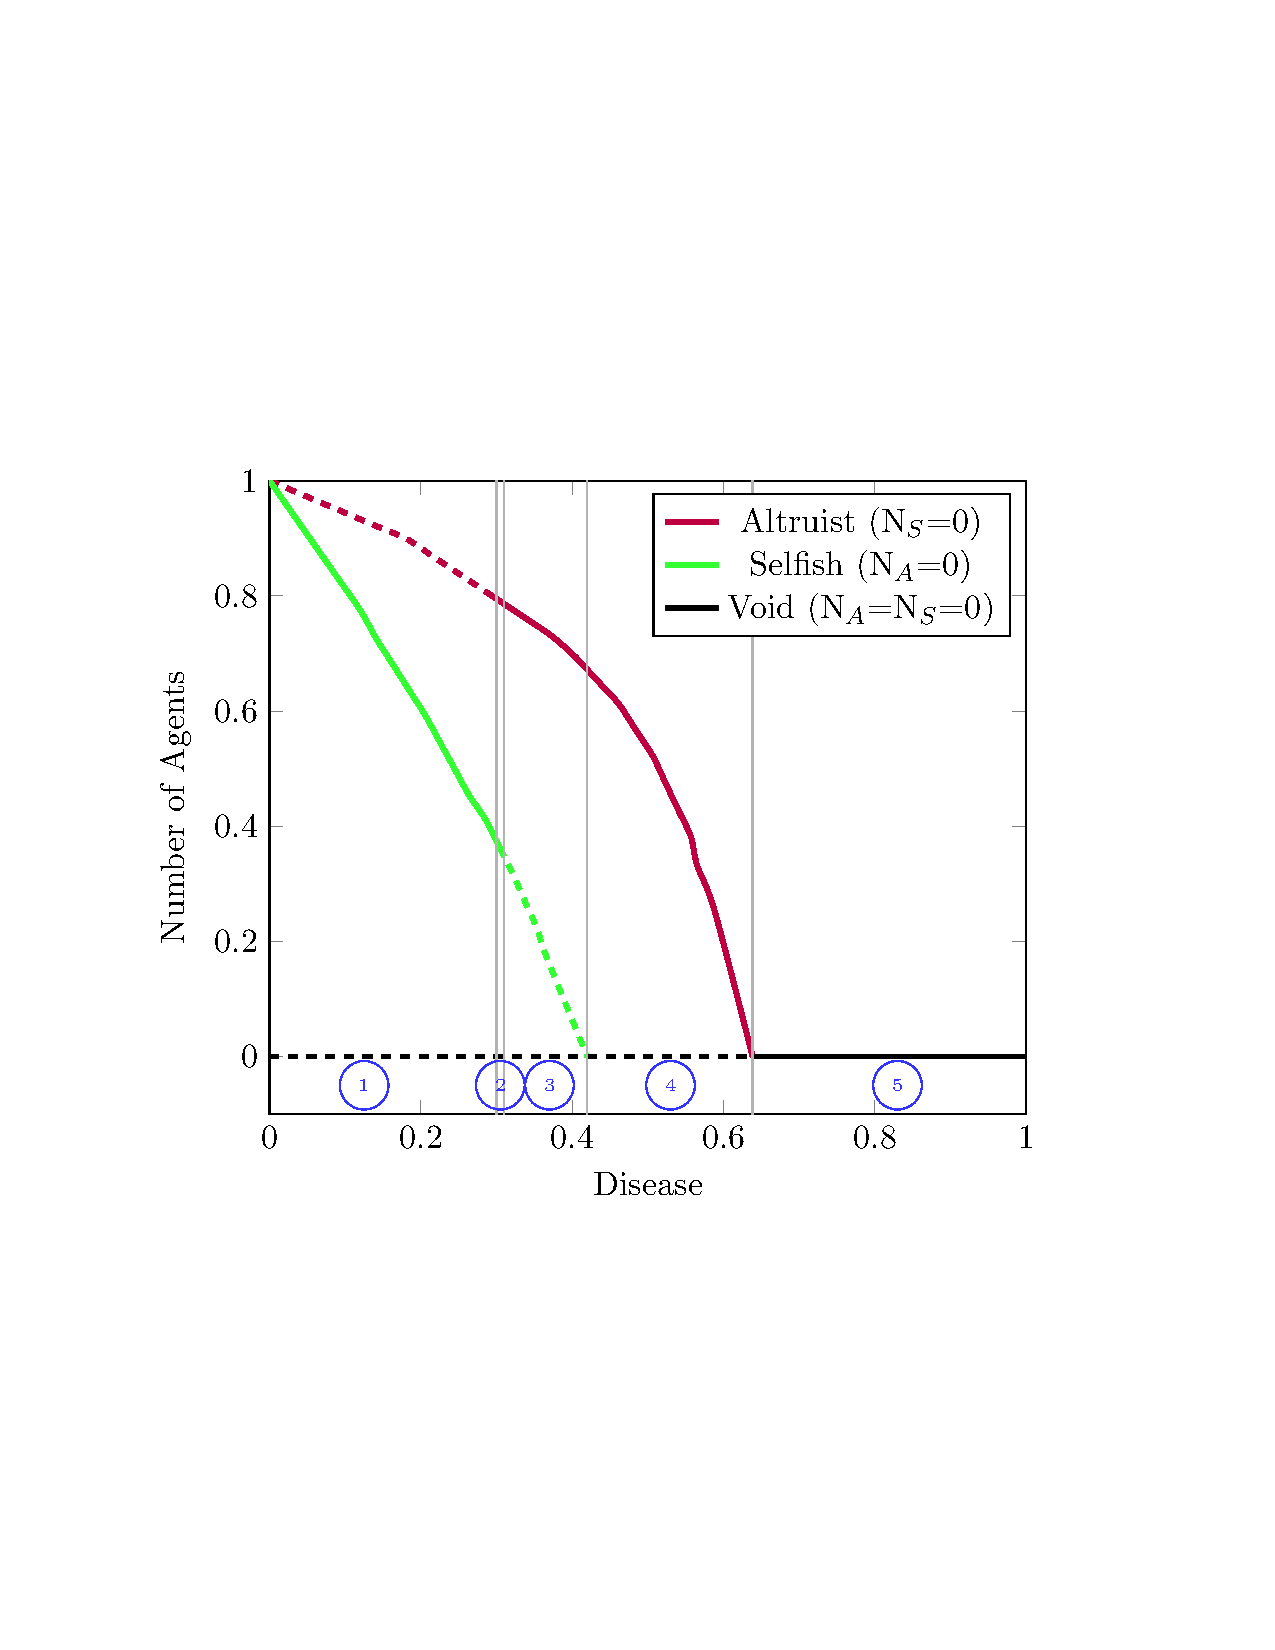
\includegraphics[width=0.75\linewidth, trim=2cm 7cm 4cm 7cm, clip=true]{Altruism}	
	\caption{Bifurcation curve for the altruism model. Stability is indicated by solid (dashed) lines for stable (unstable) branches and numbers indicate regions of behaviour separated by bifurcation points. Note region 2 occurs at a single Disease value. \label{fig:altruistBifurcation}}
\end{figure}	

	The bifurcation points in Fig.~\ref{fig:altruistBifurcation} show the Void branch inheriting the stability of the other curves. Beginning doubly unstable, the Void branch collides with the unstable Selfish branch on the boundary of regions 3 and 4. This branch remains unstable until the boundary of region 4 and 5 where it collides with the stable Altruist branch resulting in a single stable state in the system with no Altruistic or Selfish agents.
	
	Additionally the Altruistic and Selfish branches change stability in a narrow window, but at different values of Disease. In this window (region 2) there is a bifurcation where the system moves between the $N_k=0$ and $k=A,S$ planes. That is there is a branch between the Altruistic and Selfish curves in Fig.~\ref{fig:altruistBifurcation} of fixed points where both Altruistic and Selfish agents exist. Note due to the conservation of the number of agents, this branch cannot be drawn on Fig.~\ref{fig:altruistBifurcation} directly. This connecting branch is highly unstable and rapidly converges to one of the two agent branches, which are both stable in region 2. 
	
\begin{figure}[t]
	\centering 
		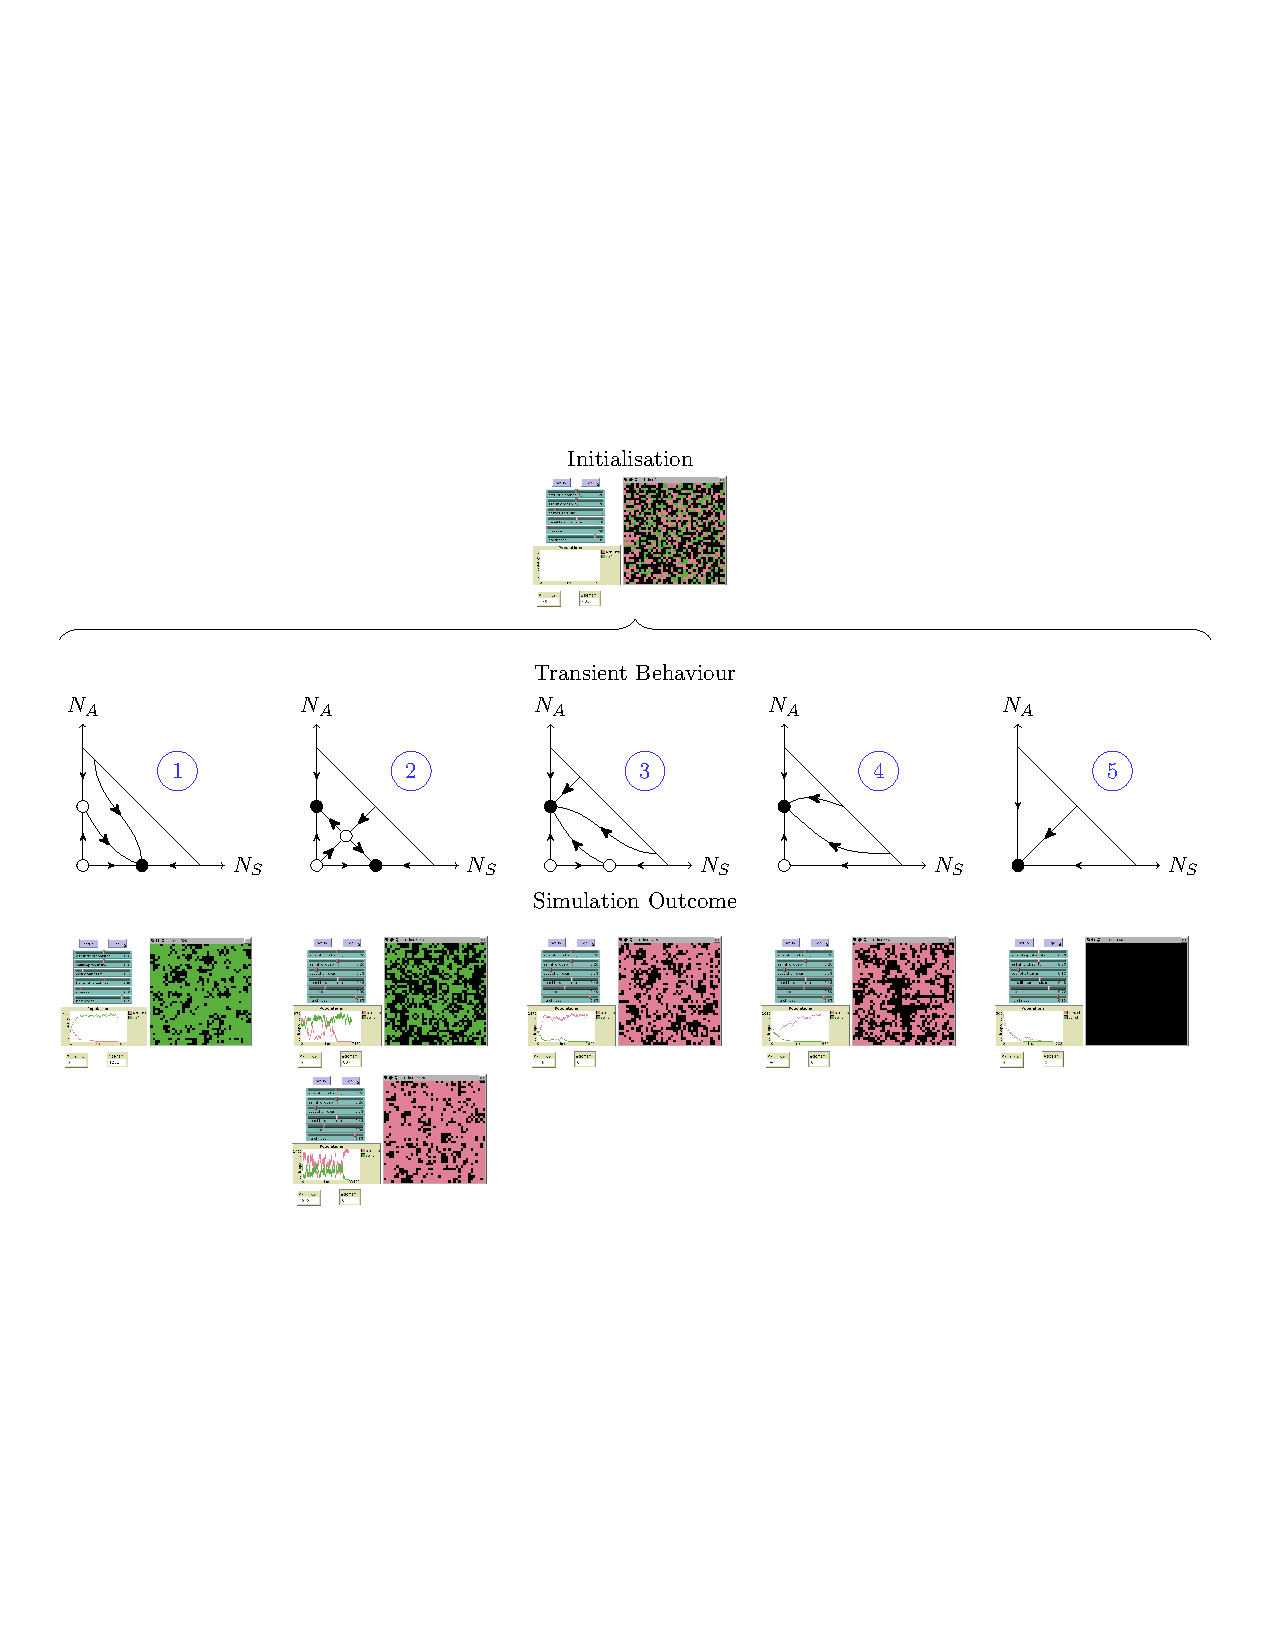
\includegraphics[width=0.9\linewidth, trim=1cm 7cm 1cm 7cm, clip=true]{AltruismSimulations}		
	\caption{Stability and Transient behaviour of altruism model in the regions in Fig.~\ref{fig:altruistBifurcation}. Agents are indicated by pink (altruists), green (selfish) and black (voids, no agent). Circles represent stable (black) and unstable (white) solutions and arrows indicate the trajectory of the dynamic behaviour. Note the origin of these plots indicate a void only state. Below each region is an example of the model behaviour under this configuration, all of which are initialised from the same settings (top), except for the value of $D$. In each case running simulations only will always converge to the stable states in regions (bottom row).  \label{fig:altruistStabillity}}
\end{figure}		
	
	The transient behaviour of the system can be better understood using Schematic diagrams of the stability in each region. Figure~\ref{fig:altruistStabillity} represents the plane in $g(N_A,N_S,N_V)$ space where the number of patches is conserved and are qualitative representations of the dynamics in the model for each region. Moreover, these diagrams also provide a clear description of the bifurcations occurring on the boundary of each region. In region 1 there are two unstable states (one doubly unstable at the origin) and a stable state consisting of only selfish agents and voids. Qualitatively we can see that system will always tend to a state where there are no Altruists, that is, the selfish agents always win out. Note that the case where $D=0$ behaves the same as in region 1, however the stable point along the $N_S$ axis and the unstable point along the $N_A$ axis are both at 1. That is in the special case where there is no Disease, agents do not die and will always converge to a full population of one agents. As $D$ is increased further the system undergoes a bifurcation as it enters region 2, with the unstable altruistic branch becoming stable and giving rise to the creation of an unstable state in between the stable altruistic and selfish branches. This fits directly with simulations in this region, where the system can converge to either of the stable branches, meaning the outcome of the battle between the two agents dependent on the initial conditions of the system. We note the lower simulation results in region 2 of Fig,~\ref{fig:altruistStabillity} where the system initially converges to the unstable state where both altruists and selfish agents exist before converging on to the stable altruist branch. Due to the level of noise in the model, and the low occurrence of convergence to this unstable state, this observation would not be possible without the knowledge of fixed points and stability obtained through the EF continuation here. Increasing $D$ further causes this new unstable state to collide with the stable state on the selfish branch making it unstable in region 3. This is an important parameter regime in the context of this model, as it is the first time that the altruists agents become `favourite' to win out over the selfish agents. From Fig.~\ref{fig:altruistStabillity} we can see that behaviour in region 3 is similar to region 1 with the altruist and selfish branches having changed stability. At the next bifurcation point, the boundary of regions 3 and 4, the now unstable selfish state collides with the void state, leaving the void branch unstable and only two fixed points in the system. Initial conditions in this region will always tend to a state with no selfish agents where only altruistic agents can survive, though they do not reach the maximum population level. The final bifurcation occurs when the only reaming stable (on the altruist Branch) collides with the unstable void state yielding a single, stable, state of the system. Regardless of initial conditions, in this region all agents will die leaving the world full of voids, which you can observe directly with Disease settings in the region. 
	
%     \begin{figure}
%        \centering
%        \begin{subfigure}[b]{0.45\textwidth}
%                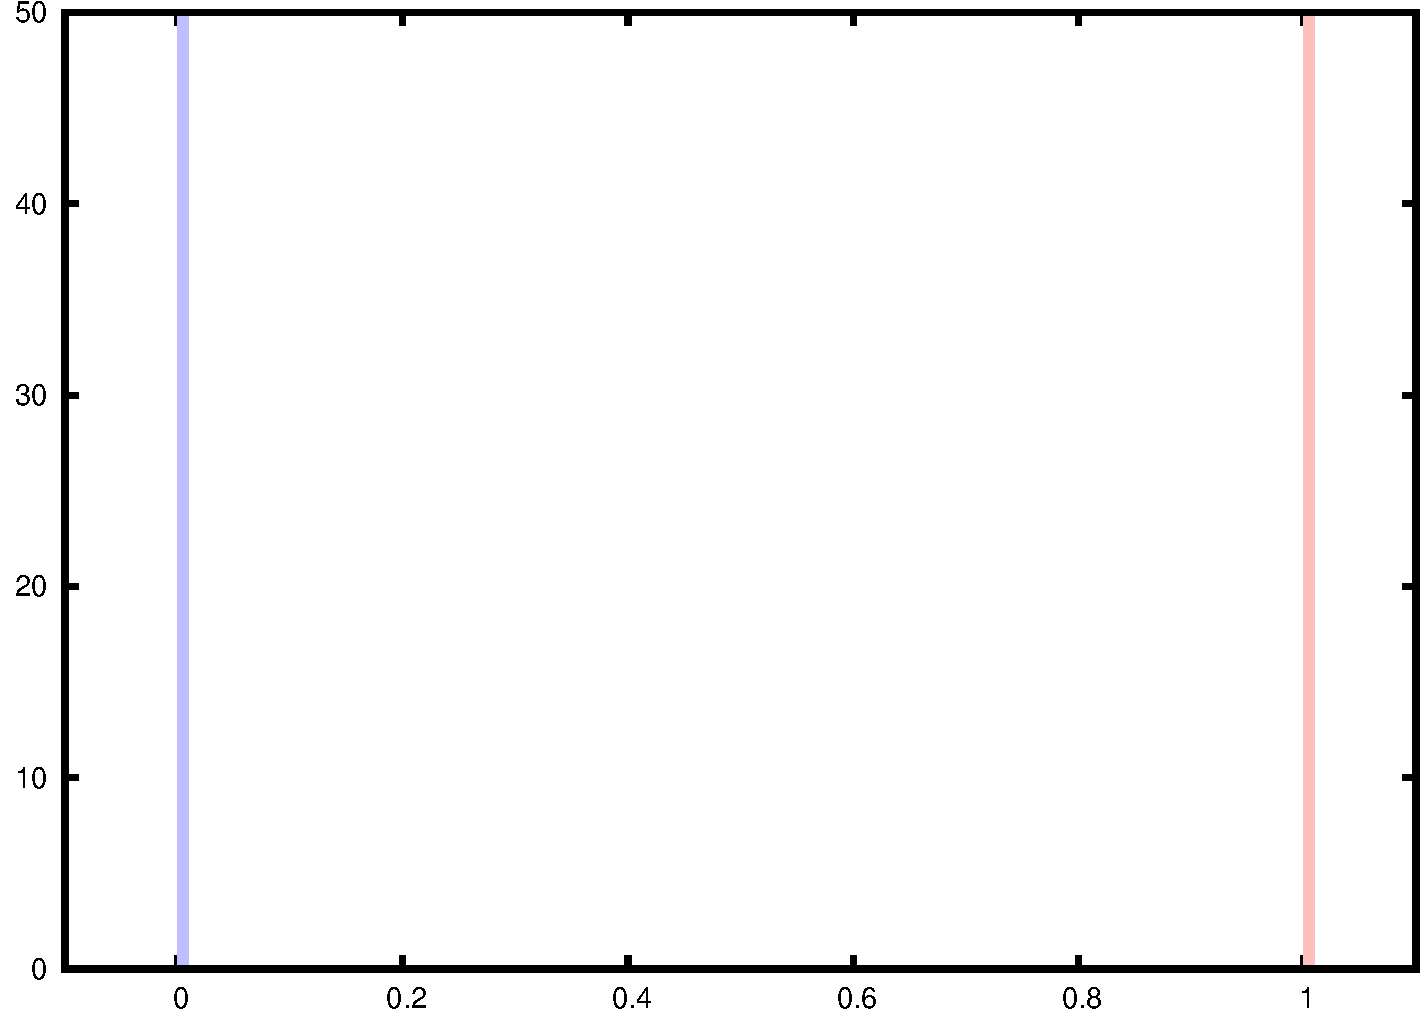
\includegraphics[page=1,width=\textwidth]{AltruismRealAlt}
%                \caption{Distribution of $N_A$ with $N_S$=0}
%        \end{subfigure}
%        \begin{subfigure}[b]{0.45\textwidth}
%                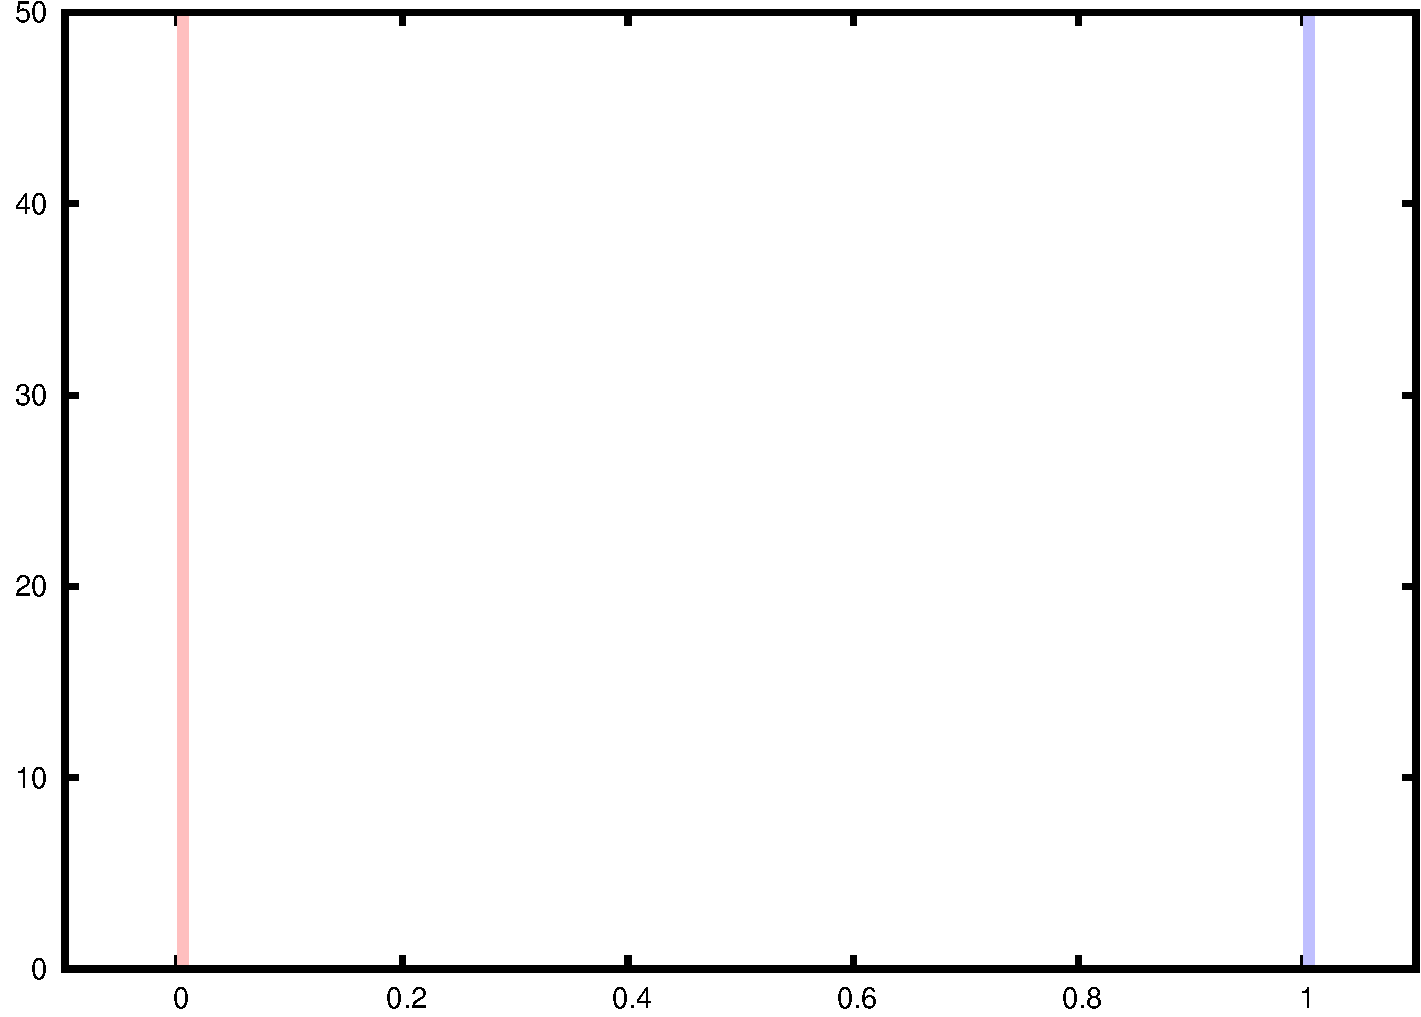
\includegraphics[page=1,width=\textwidth]{AltruismRealSel}
%                \caption{Distribution of $N_S$ with $N_A$=0}
%        \end{subfigure}\\
%        \begin{subfigure}[b]{0.45\textwidth}
%                \includegraphics[page=10,width=\textwidth]{AltruismRealAlt}
%                \caption{Distribution of $N_A$ with $N_S$=0}
%        \end{subfigure}
%        \begin{subfigure}[b]{0.45\textwidth}
%                \includegraphics[page=7,width=\textwidth]{AltruismRealSel}
%                \caption{Distribution of $N_S$ with $N_A$=0}
%        \end{subfigure}\\
%        \begin{subfigure}[b]{0.45\textwidth}
%                \includegraphics[page=20,width=\textwidth]{AltruismRealAlt}
%                \caption{Distribution of $N_A$ with $N_S$=0}
%        \end{subfigure}
%        \begin{subfigure}[b]{0.45\textwidth}
%                \includegraphics[page=16,width=\textwidth]{AltruismRealSel}
%                \caption{Distribution of $N_S$ with $N_A$=0}
%        \end{subfigure}\\
%        \caption{Continuation of the Altruism model. \label{fig:dist}}
%	\end{figure} 

 
 
 
\section{Further Reading}

The following table contains a reference list for further reading on the topic contained in this method and example. 
\begin{center}
\begin{tabular}{|l|c|}
\hline
Topic									&	Reference \\ \hline
Introduction to bifurcation analysis		&	\cite{Meunier1988}	\\
Introduction to continuation 			&	\cite{Doedel1991,Allgower1990,Rheinboldt2000,Krauskopf2007} \\ 
Introduction to equation-free methods	&	\cite{Theodoropoulos2000,Kevrekidis2003,Kevrekidis2009}	\\
Further models for altruism				&	\cite{Boyd2003, Camerer2003, Mohtashemi2003, Shultz2009, Nowak1998, Janssen2014, Janssen2014b, Janssen2008b, Pepper2007} \\
\hline
\end{tabular}
\end{center}



\section*{Acknowledgments}
{The support of the UK Engineering and Physical Sciences Research Council for programme grant EP/H021779/1 (Evolution and Resilience of Industrial Ecosystems (ERIE)) is gratefully acknowledged.}
 
 
\begin{thebibliography}{10}  

\bibitem{Netlogo}
{\sc U. Wilensky}, 
{\it NetLogo},
Center for Connected Learning and Computer-Based Modeling, Northwestern University, Evanston, IL,
http://ccl.northwestern.edu/netlogo/,
1999

\bibitem{Altruism}
{\sc U. Wilensky}, 
{\it NetLogo Altruism model},
Center for Connected Learning and Computer-Based Modeling, Northwestern University, Evanston, IL,
http://ccl.northwestern.edu/netlogo/models/Ising,
2003

\bibitem{Barkley2006}
{\sc D. Barkely, I. G. Keverekidis and A. M. Stuart},
{\it The Moment Map: Nonlinear Dynamics of Density Evolution via a Few Moments},
SIAM J. Applied Dynamical Systems, 2006, 5(3), pp 403-434

\bibitem{Avitabile2014}
{\sc D. Avitabile, R. Hoyle, G. Samaey},
{\it Noise reduction in coarse bifurcation analysis of stochastic agent-based models: an example of consumer lock-in},
SIAM Journal on Applied Dynamical System, 2014, ISSN 1536-0040 (In Press)

\bibitem{Meunier1988}
{\sc C. Meunier and A. D. Verga},
{\it Noise and Bifurcations}
J. Stat. Phys., 1988, 50(1-2), pp 345-375

\bibitem{Doedel1991}
{\sc E. Doedel, H. B. Keller and J. P. Kernevez},
{\it Numerical Analysis And Control of Bifurcation Problems (I) Bifurcation in Finite Dimensions}
Int. J. Bifurcation Chaos, 1991, 493(3), pp 493-520

\bibitem{Allgower1990}
{\sc E. L. Allgower and K. Georg},
{\it Numerical Continuation Methods, An Introduction}
Springer-Verlag Berlin Heidelberg 1990

\bibitem{Rheinboldt2000}
{\sc W. C. Rheinboldt},
{\it Numerical continuation methods: a perspective}
Journal of Computational and Applied Mathematics, 200, 124, pp 229-244

\bibitem{Krauskopf2007}
{\sc B. Krauskopf, H. M. Osinga and J. Gal\`{a}n-Vioque (Eds.)},
{\it Numerical Continuation Methods for Dynamical Systems}
Springer 2007

\bibitem{Theodoropoulos2000}
{\sc C. Theodoropoulos, Y. H. Qian and I. G. Kevrekidis IG}
{\it Coarse stability and bifurcation analysis using time-steppers: a reaction-diffusion example}
Proc. Natl. Acad. Sci. 2000, 97, pp 9840-9845

\bibitem{Kevrekidis2003}
{\sc I. G. Kevrekidis et al.} 
{\it Equation-free, coarse-grained multiscale computation: enabling microscopic simulators to perform system-level tasks}
Comm. Math. Sci. 2003, 1, pp 715-762 

\bibitem{Kevrekidis2009}
{\sc I. G. Kevrekidis and G. Samaey},
{\it Equation-Free Multiscale Computation: Algorithms and Applications},
Annual Review of Physical Chemistry, 2009, 60(1), pp 321-344

% alturist references
\bibitem{Boyd2003}
  {\sc R. Boyd, H. Gintis, S. Bowles and P. J. Richerson},
  {\it The evolution of altruistic punishment},
  Proceedings of the National Academy of Sciences, 2003, 100(6):3531-3535.
  
\bibitem{Camerer2003}
  {\sc C. F. Camerer},
  {\it Behavioral game theory: Experiments in strategic interaction},
  Russel Sage Fondation, New York, NY, 2003
  
\bibitem{Mohtashemi2003}
  {\sc M. Mohtashemi and L. Mui},
  {\it Evolution of indirect reciprocity by social information: the role of trust and reputation in evolution of altruism},
  Journal of Theoretical Biology, 2003, 223(4):523-531.   
    
\bibitem{Shultz2009}
  {\sc T. Shultz, M. Hartshorn and A. Kaznatcheev},
  {\it Why Is Ethnocentrism More Common Than Humanitarianism? },
  in Proceedings of the 31st Annual Conference of the Cognitive Science Society, 2009, pp. 2100-2105.
  
\bibitem{Nowak1998}
  {\sc M. A. Nowak and K. Sigmund},
  {\it Evolution of indirect reciprocity by image scoring},
  Nature, 1998, 393:573-577.
   
\bibitem{Janssen2014}
  {\sc M. A. Janssen and E. Ostrom},
  {\it Vulnerability of Social Norms to Incomplete Information},
  in The Complexity of Social Norms, Springer International Publishing, 2014, pp. 161-173.
  
\bibitem{Janssen2014b}
  {\sc M. A. Janssen},
  {\it The effect of social preferences on the evolution of cooperation in public good games},
  Advances in Complex Systems, 2014, 17(03n04):1450015.
   
\bibitem{Janssen2008b}
  {\sc M. A. Janssen and C. Bushman},
  {\it Evolution of cooperation and altruistic punishment when retaliation is possible }, 
  Journal of Theoretical Biology, 2008, 254(3):541-545
 
\bibitem{Pepper2007}
  {\sc J. W. Pepper},
  {\it Simple Models of Assortment through Environmental Feedback},
  Artificial Life, 2007, 13(1):1-9.


\end{thebibliography} 

\end{document} 

